\chapter{Experimentos}
En esta sección se recogen los experimentos a los que se han sometido los tres agentes introducidos en el capítulo anterior. Tras una explicación del experimento se analizarán los resultados obtenidos.
\section{Experimento individual}
La finalidad de este experimento fue la de comprobar que los mecanismos sensoriales, motores y de plasticidad homeostática del agente individual (o ``Agente 0'') funcionaban correctamente. Este experimento fue un paso previo
al desarrollo de los agentes con comportamientos colectivos. El agente sometido a este experimento fue el ``Agente 0'' que mejor puntuación obtuvo en el proceso de evolución mediante el algoritmo genético. Su puntuación fitness fue
de 0.81.

El experimento consistía (de manera similar a la función fitness individual) en situar al agente en el punto $(0,0)$ del espacio e ir mostrando de una en una 6 luces. No más de una luz puede estar encendida al mismo tiempo, la cual permanece en el espacio durante un número
de iteraciones elegidas aleatoriamente del intervalo $[0.75T, 1.25T]$, teniendo $T=1600$. Cuando una luz se apaga, se genera otra a una distancia $D \in [10R:25R]$ de la posición actual del agente, siendo $R$ el radio del agente. La intensidad ($I$) que emite la luz se elige en el momento de su creación aleatoriamente de manera que
$I = [500, 1500]$.

Durante la ejecución del experimento se guardan las posiciones por las que el agente pasa durante la ejecución del mismo.
\subsection{Resultados del Agente 0}
En este experimento el resultado importante a analizar es la trayectoria efectuada por el agente durante la realización del mismo, con la finalidad de comprobar que su comportamiento de fototaxis es el adecuado. Como puede observarse en la figura \ref{fig:agente0Trayectoria}, el agente se desplaza a la luz activa en cada momento
y se mantiene cerca de ella hasta que se apaga.

\begin{figure}[H]
    \centering
    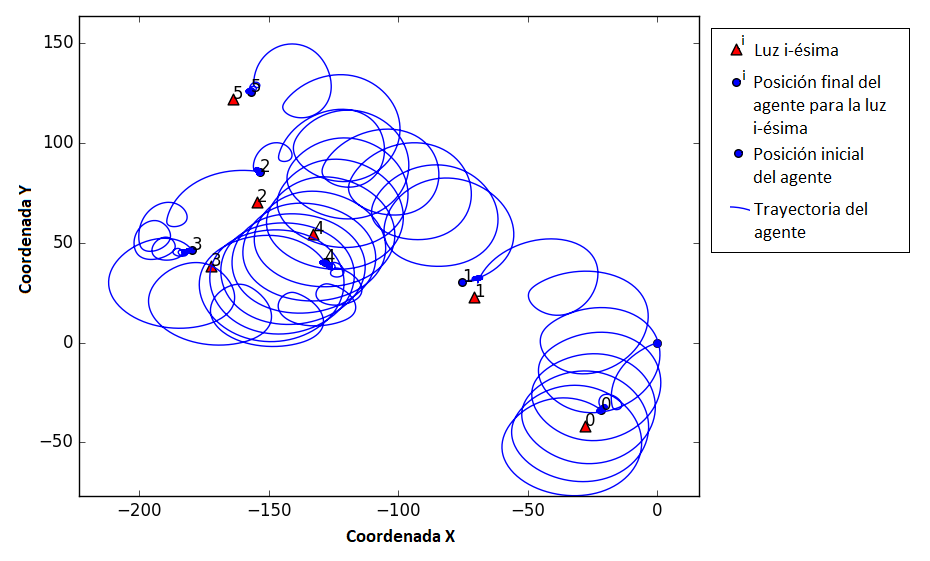
\includegraphics[width=0.8\textwidth,height=7cm]{Imagenes/Agente0Trayectoria}
    \caption{Trayectoria del ``Agente 0'' durante la realización del experimento individual.}
    \label{fig:agente0Trayectoria}
\end{figure}

Dado por comprobado el correcto funcionamiento del agente individual, se prorcedió a experimentar con los agentes colectivos.

\section{Experimento colectivo}
La finalidad de este experimento recae en comprobar, para los dos tipos tipos de agentes colectivos (``Agentes 1'' y ``Agentes 2'') un correcto comportamiento de fototaxis con restricciones colectivas. El ``Agente 1'' que participa en el experimento es el que mayor puntuación fitness ha obtenido durante su evolucón, la cual
ha sido de 0.427 tras un periodo de 10 horas de evolución. En el caso del ``Agente 2'', se ha alcanzado una fitness de 0.591 tras 10 horas de evolución. Para ambos tipos de agente, el experimento consta de tres partes:

En la primera parte, el experimento consiste (de manera similar a la función fitness colectiva) en situar al conjunto de 5 agentes del tipo que se quiere analizar a una determinada distancia del punto $(0,0)$ del espacio, que se selecciona de forma aleatoria del intervalo $[4R, 8R]$ siendo $R$ el radio del agente, y con una orientación también aleatoria.
Una vez situados, de igual manera que en el experimento individual, 6 luces irian apareciendo de forma progresiva (teniendo sólamente una activada a la vez), sólo que esta vez en vez de aparecer a una determinada distancia del agente aparecen a una distancia $D \in [10R, 25R]$ del centroide
formado por los agentes, siendo $R$ el radio del agente. Además, los agentes con comportamientos colectivos perciben al resto de agentes de forma similar a como perciben las luces (cada agente tiene una intensidad que en función de la distancia a la que se encuentre del sensor que lo lee producirá una señal
más fuerte o más suave). La intensidad ($I_{agente})$ que emite cada agente es un valor fijo $I_{agente} = 750$.

Durante la ejecución de esta parte del experimento se guardan las trayectorias de los 5 agentes y los valores de las activaciones de las 6 neuronas de cada uno de los agentes durante cada iteración de la ejecución.

La segunda parte del experimento consiste en añadir cierto ruido a las señales de lectura de los sensores luminosos y colectivos, para analizar el impacto que este ruido tiene en la puntuación fitness del experimento. Por ello, para esta parte, se calcula la puntuación fitness de la ejecución de manera exactamente igual a la de la función fitness colectiva
utilizada durante la evolución de los agentes.

El ruido $R$ de cada señal $S$ se calcula mediante la fórmula \ref{eq:eqRuido}, donde $\alpha$ es el factor de ruido. Para este experimento se han analizado las variaciones en la fitness ante la presencia de ruido con unos valores $\alpha$ de 0, 0.2, 0.34 y 0.44.
\begin{equation} \label{eq:eqRuido}
 \centering
R = \alpha S
\end{equation}

La señal final $S_{f}$ (posterior a la aplicación de ruido) de cada uno de los sensores se calcula mediante la fórmula \ref{eq:formulaRuido}, donde $S$ representa la señal leída por los sensores y $R$ representa el ruido aplicado a esa señal. El término $rand(a,b)$ representa un valor elegido aleatoriamente del rango $[a,b]$.

\begin{equation} \label{eq:formulaRuido}
 \centering
S_{f} = \text{rand}(S - R, S + R)
\end{equation}

Para esta parte del experimento se han guardado las puntuaciones fitness obtenidas en 30 ejecuciones para cada nivel de ruido.

En la tercera parte del experimento, se añade ruido (de forma similar a la segunda parte), pero, esta vez, primero a los ritmos de plasticidad y después a los pesos de las conexiones sinápticas entre las neuronas, para comprobar la robustez de cada uno de los agentes frente a estas perturbaciones. Al igual que en el apartado dos, se tomarán 30 mediciones de la fitness resultante de la ejecución
para cada nivel de ruido.

\subsection{Resultados del Agente 1}
En esta sección se presenta el análisis de los resultados del conjunto de agentes de tipo 1 en el experimento colectivo.
\subsubsection{Trayectorias}
El análisis de las trayectorias nos permite visualizar si el comportamiento de fototaxis colectivo del grupo de agentes del tipo 1 ha sido el correcto. Como puede verse en la figura \ref{fig:agente1Trayectoria}, tres agentes (trayectorias de colores verde, azul y negro) han permanecido cerca de la fuente de luz número 4 mientras estaba activa, lo cual puede visualizarse observando
las concentraciones de circunferencias presentes en las inmediaciones de la fuente de luz. Los otros dos agentes del conjunto (trayectorias cian y roja) no se han acercado a la luz, cumpliendo de manera satisfactoria la restricción colectiva establecida (máximo 3 agentes al mismo tiempo cerca de una luz).

\begin{figure}[H]
    \centering
    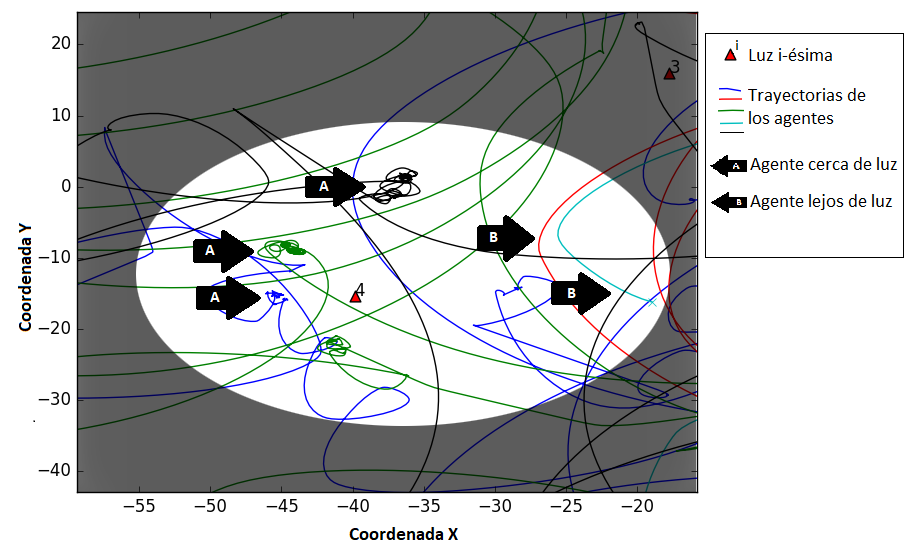
\includegraphics[width=0.9\textwidth,height=8cm]{Imagenes/Agente1Trayectoria}
    \caption{Fragmento de trayectorias del conjunto de agentes de tipo 1 que demuestran comportamiento de fototaxis colectiva.}
    \label{fig:agente1Trayectoria}
\end{figure}

\subsubsection{Activaciones neuronales}
Para analizar las activaciones neuronales del conjunto de agentes de tipo 1, se ha seleccionado un único agente como representante del conjunto. Las activaciones de las neuronas que componen el controlador de este agente pueden verse en la figura \ref{fig:activ1}, cuyos valores se ven representados por la línea azul. Las dos líneas horizontales negras situadas en los valores del eje Y 4 y -4 representan
el límite superior e inferior de la zona estable de la neurona.

\begin{figure}[H]
  \centering
  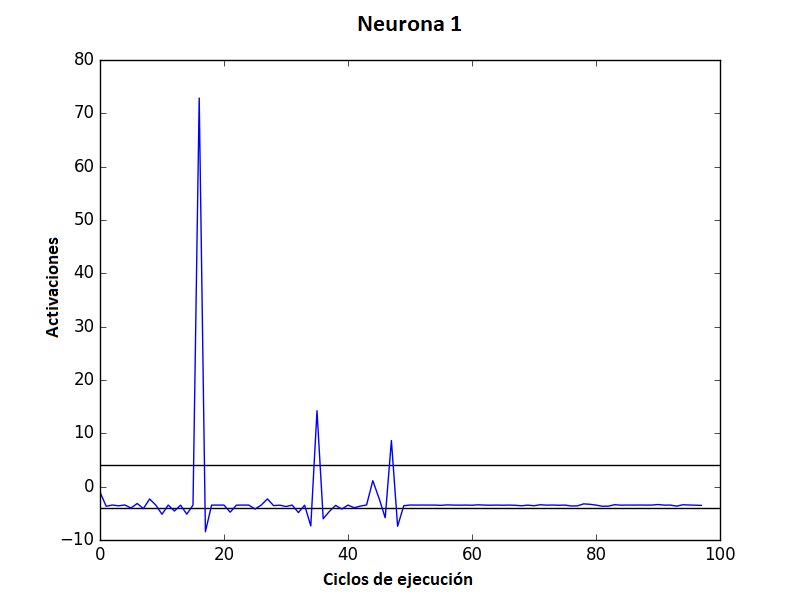
\includegraphics[width=.45\textwidth]{Imagenes/Activaciones10}\quad
  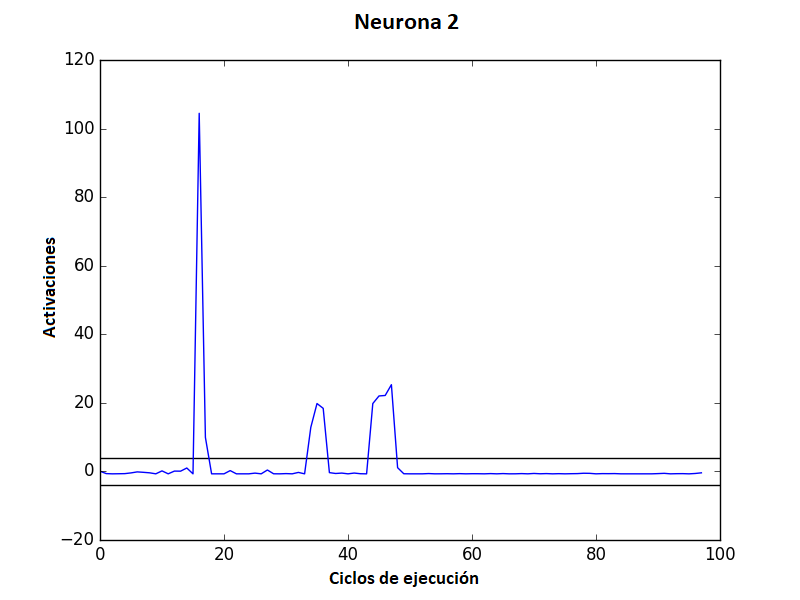
\includegraphics[width=.45\textwidth]{Imagenes/Activaciones11}
  \medskip
  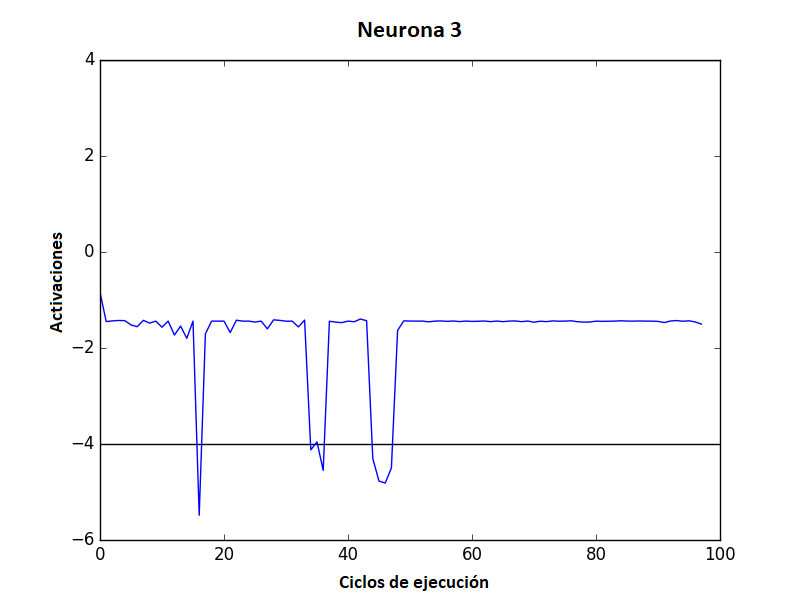
\includegraphics[width=.45\textwidth]{Imagenes/Activaciones12}\quad
  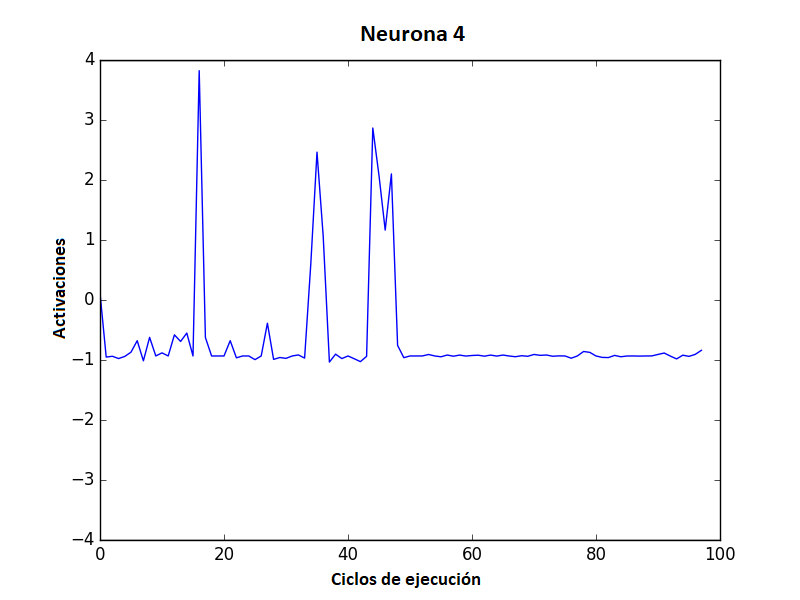
\includegraphics[width=.45\textwidth]{Imagenes/Activaciones13}
  \medskip
  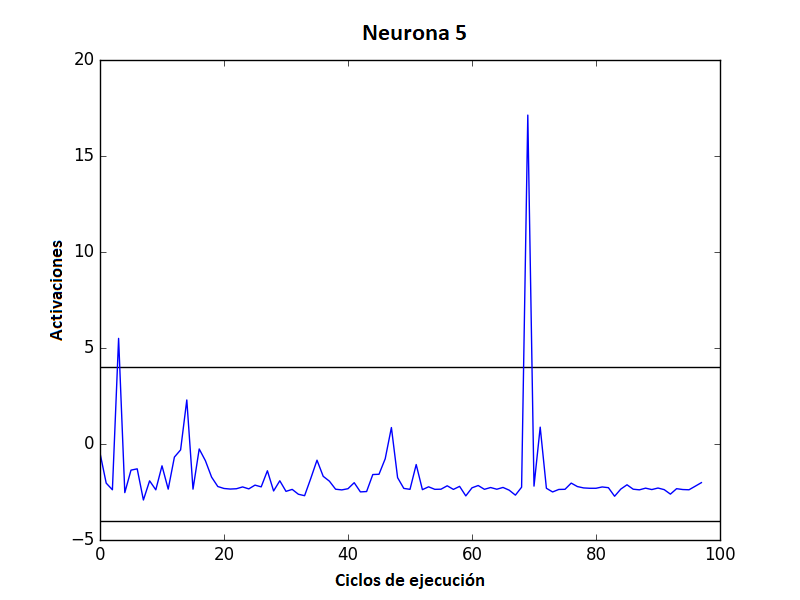
\includegraphics[width=.45\textwidth]{Imagenes/Activaciones14}\quad
  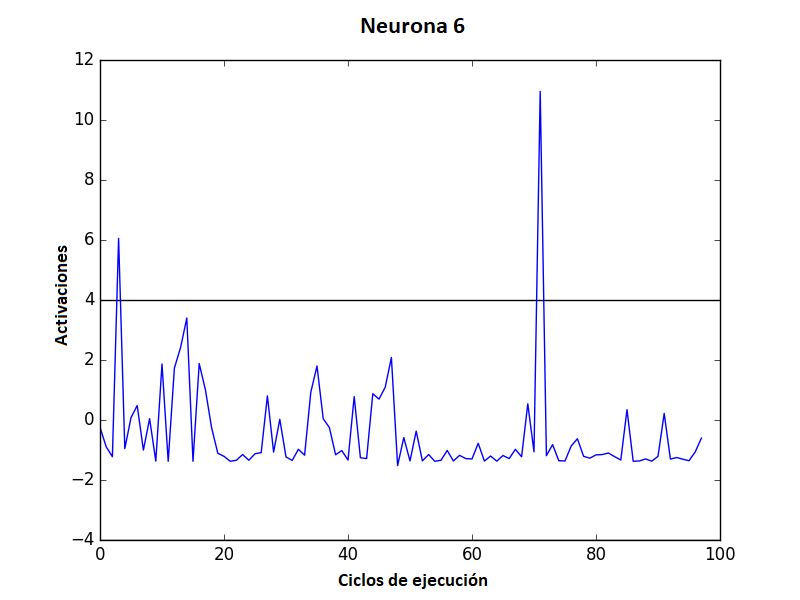
\includegraphics[width=.45\textwidth]{Imagenes/Activaciones15}

  \caption{Activaciones de las 6 neuronas del agente representativo del grupo de agentes de tipo 1.}
  \label{fig:activ1}
\end{figure}

Se ha calculado, para cada neurona de cada uno de los agentes de tipo 1 que componen el conjunto de agentes utilizados para el experimento, el área (integrando) del espacio que las activaciones de la neurona han permanecido fuera de los límites, tanto superior como inferior, de la zona de estabilidad (líneas horizontales negras de las gráficas). En la tabla \ref{table:tActivaciones1} se pueden ver
los valores de estas áreas para cada neurona de cada agente.

\begin{table}[H]
\centering
\begin{tabular}{c|cccccc}
\multicolumn{1}{l|}{}                & \multicolumn{6}{c}{\textbf{Neuronas}}                                       \\ \hline
\multicolumn{1}{l|}{\textbf{Agente}} & \textbf{1} & \textbf{2} & \textbf{3} & \textbf{4} & \textbf{5} & \textbf{6} \\ \hline
\textbf{1}                           & 2.7186     & 6.1104     & 61.468     & 480.64     & 1.089      & 0.0        \\
\textbf{2}                           & 5456.456   & 7588.078   & 34.91      & 33.783     & 36.65      & 0.0        \\
\textbf{3}                           & 43.742     & 190.657    & 53.7353    & 96.011     & 1.98       & 0.0        \\
\textbf{4}                           & 1909.514   & 2173.154   & 1.1268     & 98.664     & 34.29349   & 0.0        \\
\textbf{5}                           & 104.5142   & 218.7017   & 14.631     & 9.008      & 4.545      & 0.0
\end{tabular}
\caption{Tabla con el área que cada neurona de cada agente del conjunto de agentes de tipo 1 ha permanecido fuera de los límites de estabilidad establecidos.}
\label{table:tActivaciones1}
\end{table}

Se ha observado, que en este tipo de agentes las salidas de las activaciones neuronales de la zona estable son bastante frecuentes, pero de breve duración (el agente se recupera rápido).

La totalidad de las gráficas de las activaciones neuronales de los agentes del conjunto de agentes de tipo 1 se encuentra en el Anexo \ref{ch:anexo3}.

\subsubsection{Robustez ante ruido en los sensores}
Como se ha explicado anteriormente, para cada nivel de ruido se han tomado 30 mediciones de los resultados fitness obtenidos en la ejecución del experimento. El objetivo es analizar la robustez (consistencia frente al ruido en los sensores) del conjunto de agentes. Las mediciones obtenidas se han representado en forma de diagramas de caja para visualizar su distribución (figura \ref{fig:boxPlot1}).

\begin{figure}[H]
    \centering
    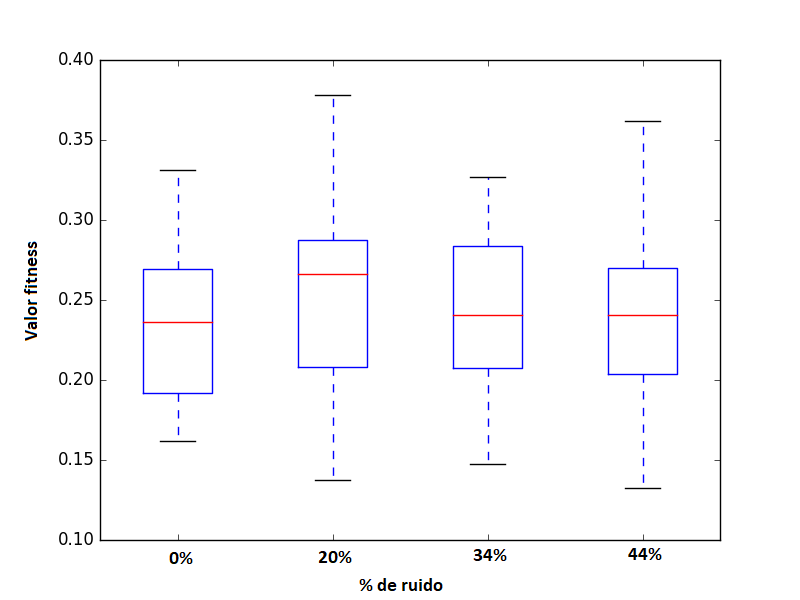
\includegraphics[width=0.8\textwidth,height=8cm]{Imagenes/BoxPlot1}
    \caption{Diagramas de caja para las mediciones de la fitness en presencia de ruido en los sensores de los agentes de tipo 1.}
    \label{fig:boxPlot1}
\end{figure}

Además, para aumentar la rigurosidad, se ha efectuado un test de \textit{t de Student} para cada par de población de mediciones, para comprobar si las medias de las dos poblaciones de datos examinadas (de tamaño pequeño y con distribución normal) pueden considerarse iguales. Los pares de poblaciones probados han sido: sin ruido y 0.2, sin ruido y 0.34, sin ruido y 0.44. Los resultados del test pueden verse en la tabla \ref{table:tAgente1}.

\begin{table}[H]
\centering
\begin{tabular}{llc}
\multicolumn{3}{c}{\textbf{Test t-Student para Agente 1}}                                                                                                    \\ \hline
\multicolumn{2}{l|}{\textbf{\begin{tabular}[c]{@{}l@{}}Población de mediciones\\ comparadas\end{tabular}}} & \multicolumn{1}{l}{\textbf{p-valor obtenido}}   \\ \hline
\multicolumn{2}{l}{Sin ruido - 0.2}                                                                        & 0.075                                            \\
\multicolumn{2}{l}{Sin ruido - 0.34}                                                                       & 0.39                                            \\
\multicolumn{2}{l}{Sin ruido - 0.44}                                                                       & 0.54
\end{tabular}
\caption{P-valores obtenidos de la ejecución del test \textit{t de Student} sobe los pares de poblaciones de mediciones obtenidas.}
\label{table:tAgente1}
\end{table}

Al obtener, para todos los pares de poblaciones, un \textit{p-valor} mayor que $0.05$ se confirma la hipótesis de que las medias pueden considerarse iguales y, por tanto, que el ruido en los sensores no afecta de manera significativa a la puntuación
de los agentes de tipo 1.


\subsubsection{Robustez ante ruido en parámetros de la plasticidad}
Para comprobar la robustez de este tipo de agentes ante presencia de perturbaciones que afecten a la plasticidad se ha probado a añadir ruido a dos parámetros involucrados en los mecanismos de plasticidad.
Primero, se ha aplicado ruido a los ritmos de plasticidad de las neuronas de los agentes, guardando los valores fitness resultantes de ejecutar el experimento con presencia de dicho ruido. Los niveles de ruido probados,
al igual que en el caso de los sensores, han sido de 0, 0.2, 0.34 y 0.44. Para cada nivel de ruido se han medido 30 puntuaciones fitness. Estas mediciones se han representado en forma de diagramas de caja para visualizar su distribución (figura \ref{fig:boxPlotNP1}).

\begin{figure}[H]
    \centering
    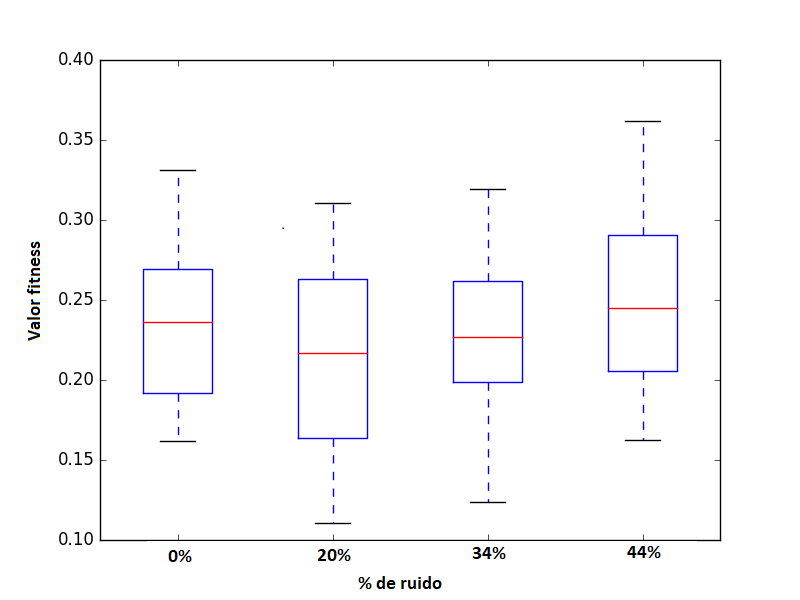
\includegraphics[width=0.8\textwidth,height=8cm]{Imagenes/BoxPlotNP1}
    \caption{Diagramas de caja para las mediciones de la fitness en presencia de ruido en los ritmos de plasticidad de los agentes de tipo 1.}
    \label{fig:boxPlotNP1}
\end{figure}

Además, para aumentar la rigurosidad, se ha efectuado un test de \textit{t de Student} para cada par de población de mediciones, para comprobar si las medias de las dos poblaciones de datos examinadas (de tamaño pequeño y con distribución normal) pueden considerarse iguales. Los pares de poblaciones probados han sido: sin ruido y 0.2, sin ruido y 0.34, sin ruido y 0.44. Los resultados del test pueden verse en la tabla \ref{table:tAgenteNP1}.

\begin{table}[H]
\centering
\begin{tabular}{llc}
\multicolumn{3}{c}{\textbf{Test t-Student para Agente 1}}                                                                                                    \\ \hline
\multicolumn{2}{l|}{\textbf{\begin{tabular}[c]{@{}l@{}}Población de mediciones\\ comparadas\end{tabular}}} & \multicolumn{1}{l}{\textbf{p-valor obtenido}}   \\ \hline
\multicolumn{2}{l}{Sin ruido - 0.2}                                                                        & 0.15                                            \\
\multicolumn{2}{l}{Sin ruido - 0.34}                                                                       & 0.52                                            \\
\multicolumn{2}{l}{Sin ruido - 0.44}                                                                       & 0.25
\end{tabular}
\caption{P-valores obtenidos de la ejecución del test \textit{t de Student} sobe los pares de poblaciones de mediciones obtenidas.}
\label{table:tAgenteNP1}
\end{table}

Al obtener, para todos los pares de poblaciones, un \textit{p-valor} mayor que $0.05$ se confirma la hipótesis de que las medias pueden considerarse iguales y, por tanto, que el ruido en los ritmos de plasticidad no afecta de manera significativa a la puntuación
de los agentes de tipo 1.

Por último, se ha aplicado ruido a los pesos de las conexiones sinápticas de las neuronas, durante el proceso de plasticidad, guardando los valores fitness resultantes de ejecutar el experimento con presencia de dicho ruido. Los niveles de ruido probados,
de nuevo, han sido de 0, 0.2, 0.34 y 0.44. Para cada nivel de ruido se han medido 30 puntuaciones fitness. Estas mediciones se han representado en forma de diagramas de caja para visualizar su distribución (figura \ref{fig:boxPlotNW1}).

\begin{figure}[H]
    \centering
    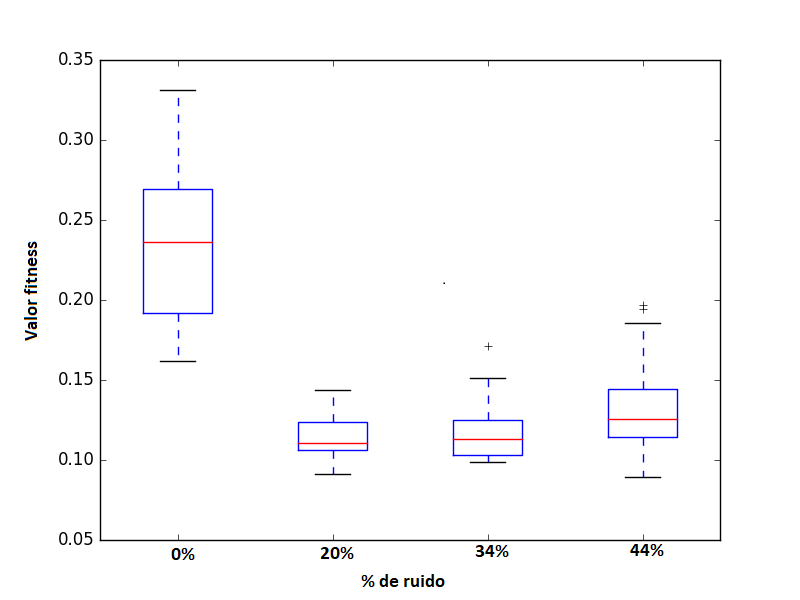
\includegraphics[width=0.8\textwidth,height=8cm]{Imagenes/BoxPlotNW1}
    \caption{Diagramas de caja para las mediciones de la fitness en presencia de ruido en los pesos sinápticos de los agentes de tipo 1.}
    \label{fig:boxPlotNW1}
\end{figure}

De nuevo, para aumentar la rigurosidad, se ha efectuado un test de \textit{t de Student} para cada par de población de mediciones, con el fin de comprobar si las medias de las dos poblaciones de datos examinadas (de tamaño pequeño y con distribución normal) pueden considerarse iguales.
Los pares de poblaciones probadas han sido: sin ruido y 0.2, sin ruido y 0.34, sin ruido y 0.44. Los resultados del test pueden verse en la tabla \ref{table:tAgenteNW1}.

\begin{table}[H]
\centering
\begin{tabular}{llc}
\multicolumn{3}{c}{\textbf{Test t-Student para Agente 1}}                                                                                                    \\ \hline
\multicolumn{2}{l|}{\textbf{\begin{tabular}[c]{@{}l@{}}Población de mediciones\\ comparadas\end{tabular}}} & \multicolumn{1}{l}{\textbf{p-valor obtenido}}   \\ \hline
\multicolumn{2}{l}{Sin ruido - 0.2}                                                                        & 0.000000011                                            \\
\multicolumn{2}{l}{Sin ruido - 0.34}                                                                       & 0.00000002                                            \\
\multicolumn{2}{l}{Sin ruido - 0.44}                                                                       & 0.000001744
\end{tabular}
\caption{P-valores obtenidos de la ejecución del test \textit{t de Student} sobe los pares de poblaciones de mediciones obtenidas.}
\label{table:tAgenteNW1}
\end{table}

Al obtener, para todos los pares de poblaciones, un \textit{p-valor} menor que $0.05$ se rechaza la hipótesis de que las medias pueden considerarse iguales y por tanto, se asume que el ruido en los pesos sinápticos afecta de manera significativa a la puntuación
de los agentes de tipo 1.

\subsection{Resultados del Agente 2}
En esta sección se presenta el análisis de los resultados del conjunto de agentes de tipo 2 en el experimento colectivo.
\subsubsection{Trayectorias}
El análisis de las trayectorias nos permite visualizar si el comportamiento de fototaxis colectivo del grupo de agentes de tipo 2 ha sido el correcto. Como puede verse en la figura \ref{fig:agente2Trayectoria}, tres agentes (trayectorias de colores verde, azul y rojo) han permanecido cerca de la fuente de luz número 5 mientras estaba activa, lo cual puede visualizarse observando
las concentraciones de circunferencias cerradas presentes en las inmediaciones de la fuente de luz. Los otros dos agentes del conjunto (trayectorias cian y negra) no se han acercado a la luz, cumpliendo de manera satisfactoria la restricción colectiva establecida (máximo 3 agentes al mismo tiempo cerca de una luz).

\begin{figure}[H]
    \centering
    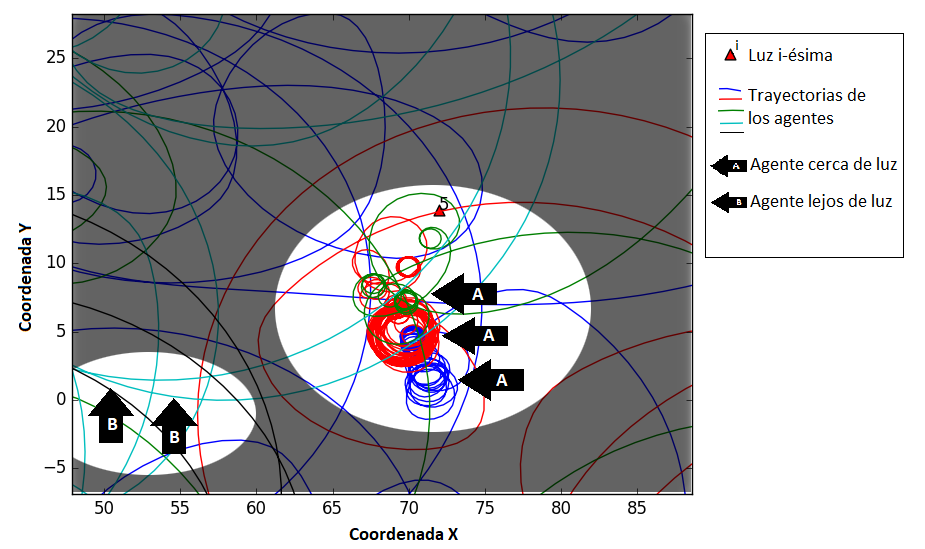
\includegraphics[width=0.9\textwidth,height=7cm]{Imagenes/Agente2Trayectoria}
    \caption{Fragmento de trayectorias del conjunto de agentes de tipo 2 que demuestran comportamiento de fototaxis colectiva.}
    \label{fig:agente2Trayectoria}
\end{figure}

\subsubsection{Activaciones neuronales}
Para analizar las activaciones del conjunto de agentes de tipo 2, se ha seleccionado un único agente como representante del conjunto. Las activaciones de las neuronas que componen el controlador de este agente pueden verse en la figura \ref{fig:activ2}, cuyos valores se ven representados por la línea azul. Las dos líneas horizontales negras situadas en los valores del eje Y 4 y -4 representan
el límite superior e inferior de la zona estable de la neurona.

\begin{figure}[H]
  \centering
  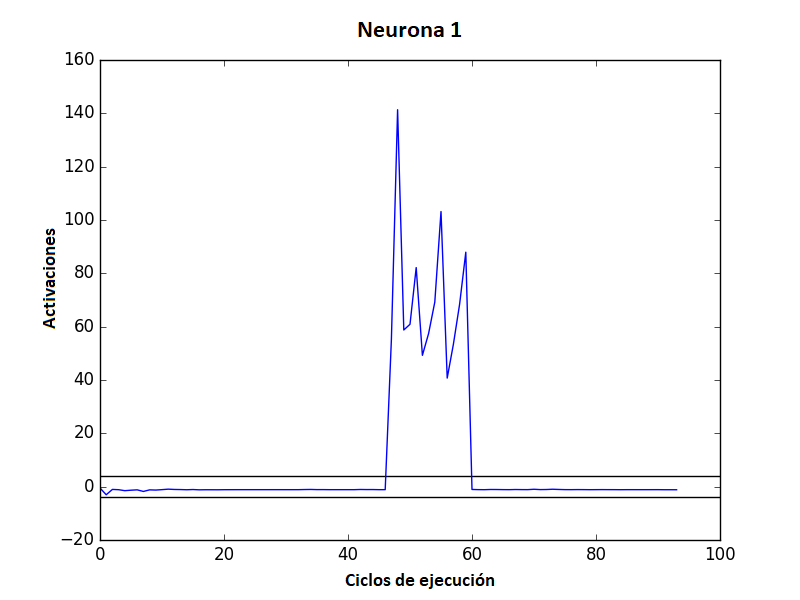
\includegraphics[width=.45\textwidth]{Imagenes/Activaciones20}\quad
  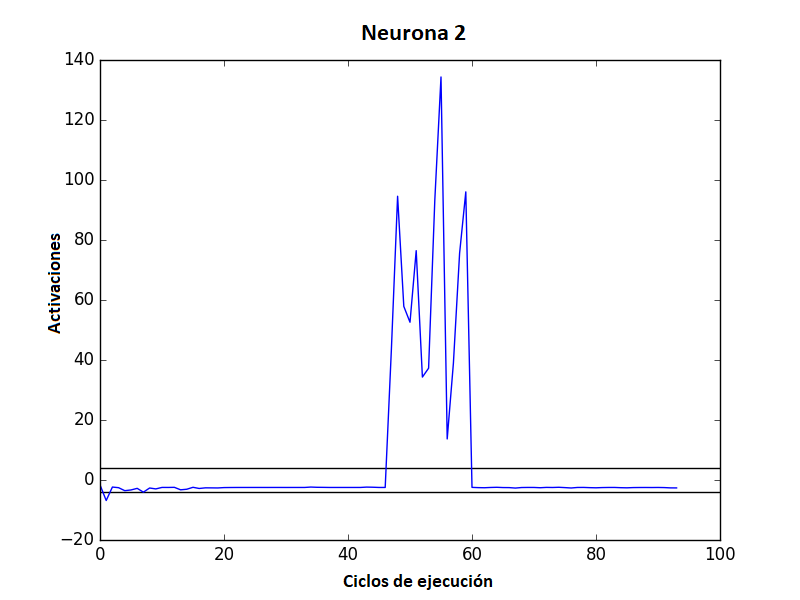
\includegraphics[width=.45\textwidth]{Imagenes/Activaciones21}
  \medskip
  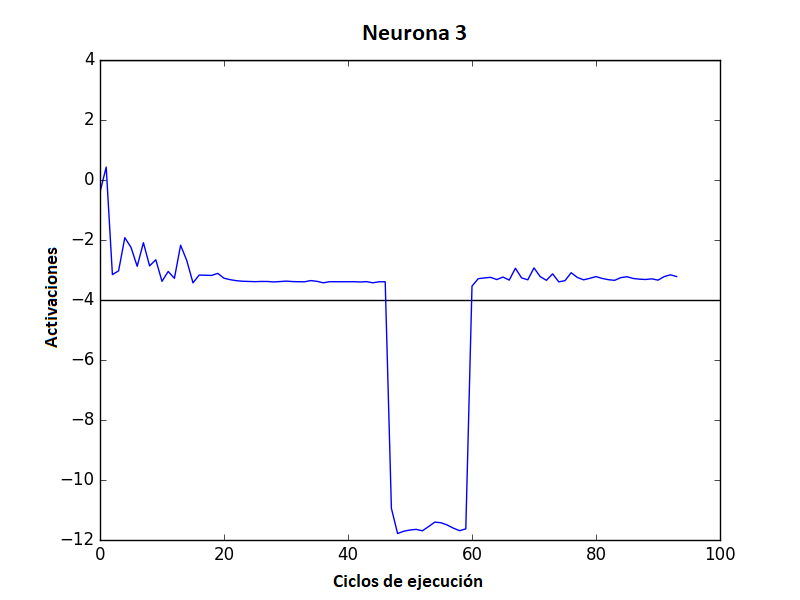
\includegraphics[width=.45\textwidth]{Imagenes/Activaciones22}\quad
  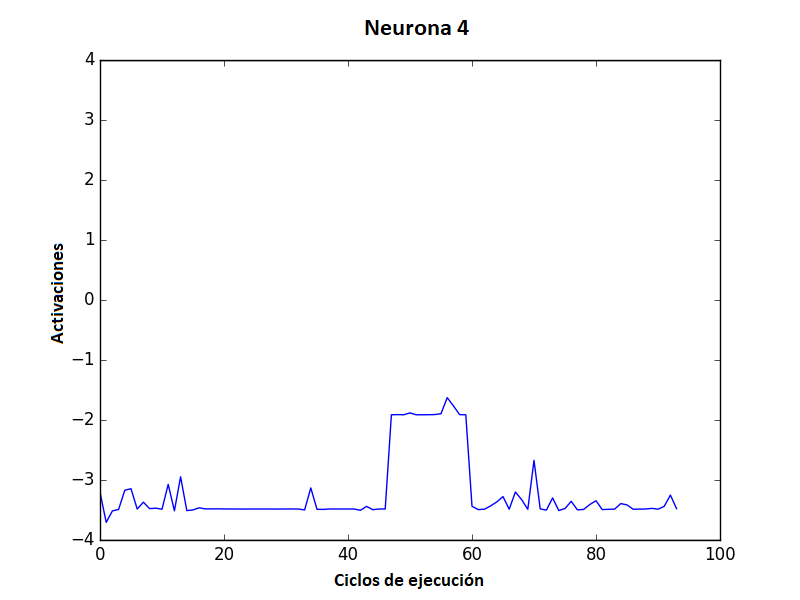
\includegraphics[width=.45\textwidth]{Imagenes/Activaciones23}
  \medskip
  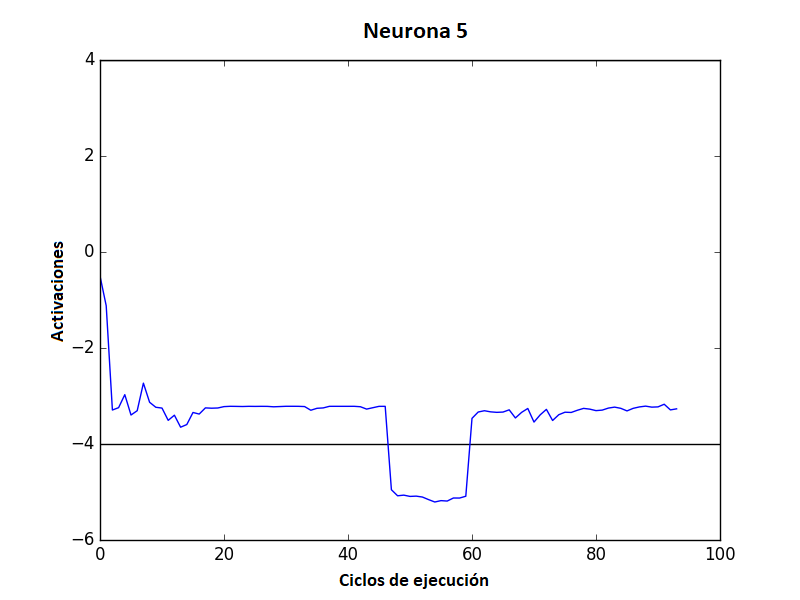
\includegraphics[width=.45\textwidth]{Imagenes/Activaciones24}\quad
  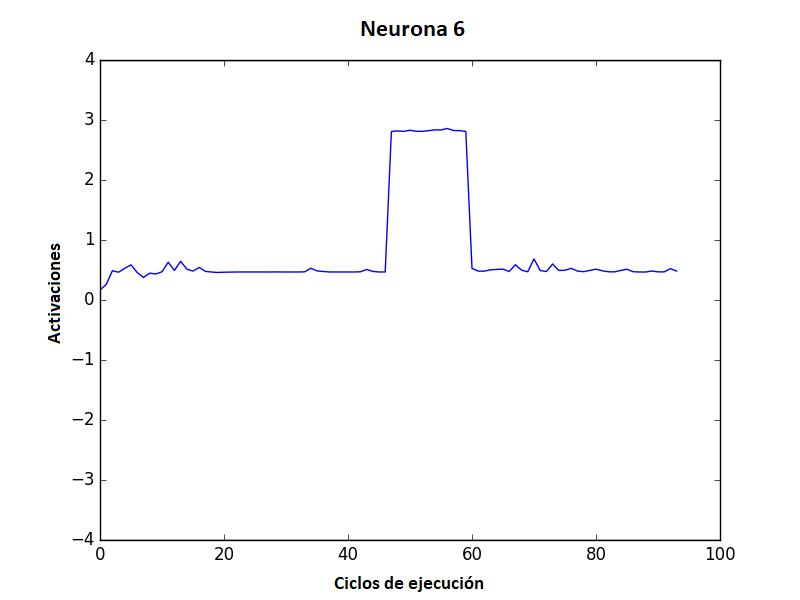
\includegraphics[width=.45\textwidth]{Imagenes/Activaciones25}

  \caption{Activaciones de las 6 neuronas del agente representativo del grupo de agentes de tipo 2.}
  \label{fig:activ2}
\end{figure}

Se ha calculado, para cada neurona de cada uno de los agentes de tipo 2 que componen el conjunto de agentes utilizados para el experimento, el área (integrando) del espacio que las activaciones de la neurona han permanecido fuera de los límites, tanto superior como inferior, de la zona de estabilidad (líneas horizontales negras de las gráficas). En la tabla \ref{table:tActivaciones2} se pueden ver
los valores de estas áreas para cada neurona de cada agente.

\begin{table}[H]
\centering
\begin{tabular}{c|cccccc}
\multicolumn{1}{l|}{}                & \multicolumn{6}{c}{\textbf{Neuronas}}                                       \\ \hline
\multicolumn{1}{l|}{\textbf{Agente}} & \textbf{1} & \textbf{2} & \textbf{3} & \textbf{4} & \textbf{5} & \textbf{6} \\ \hline
\textbf{1}                           & 875.9847   & 799.4      & 98.248     & 0.0        & 14.455     & 0.0        \\
\textbf{2}                           & 1291.039   & 828.222    & 31644.64   & 5919.85    & 109.994    & 0.0        \\
\textbf{3}                           & 0.0        & 5.1314     & 0.0        & 0.0        & 0.3        & 0.0        \\
\textbf{4}                           & 7119.155   & 19108.05   & 7203.446   & 7052.342   & 98.927     & 0.0        \\
\textbf{5}                           & 5770.375   & 4217.139   & 6793.95    & 26173.23   & 50.245     & 0.0
\end{tabular}
\caption{Tabla con el área que cada neurona de cada agente del conjunto de agentes de tipo 2 ha permanecido fuera de los límites de estabilidad establecidos.}
\label{table:tActivaciones2}
\end{table}

Se ha observado, que en este tipo de agentes las salidas de las activaciones de la zona estable son poco frecuentes, pero suelen tener una duración elevada (el agente tarda en recuperarse).

La totalidad de las gráficas de las activaciones de las neuronas del conjunto de agentes de tipo 2 se encuentra en el Anexo \ref{ch:anexo4}.
\subsubsection{Robustez ante ruido en los sensores}
Como se ha explicado anteriormente, para cada nivel de ruido se han tomado 30 mediciones de los resultados fitness obtenidos en la ejecución del experimento. El objetivo es analizar la robustez (consistencia frente al ruido) del conjunto de agentes. Las mediciones obtenidas se han representado en forma de diagramas de caja para visualizar su distribución (figura \ref{fig:boxPlot2}).

\begin{figure}[H]
    \centering
    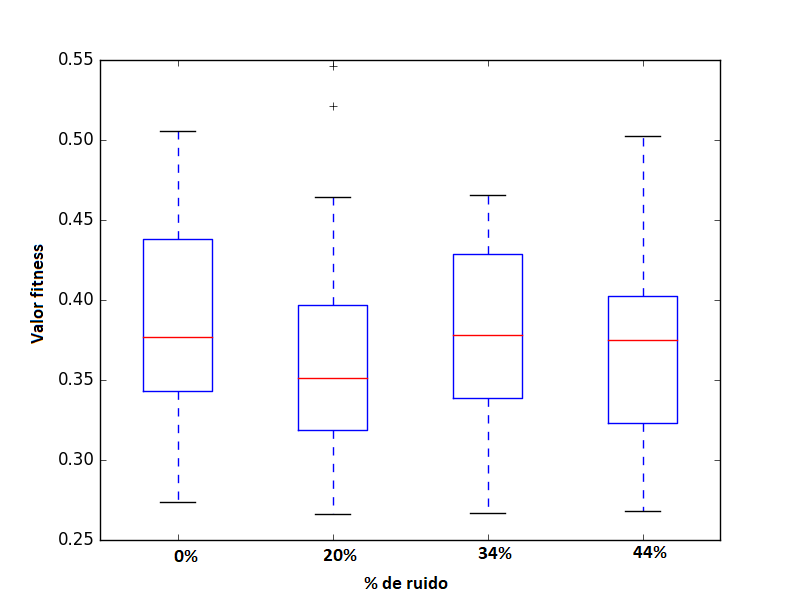
\includegraphics[width=0.8\textwidth,height=8cm]{Imagenes/BoxPlot2}
    \caption{Diagramas de caja para las mediciones de la fitness en presencia de ruido en los sensores de los agentes de tipo 2.}
    \label{fig:boxPlot2}
\end{figure}

Además, para aumentar la rigurosidad, se ha efectuado un test de \textit{t de Student} para cada par de población de mediciones, con el fin de comprobar si las medias de las dos poblaciones de datos examinadas (de tamaño pequeño y con distribución normal) pueden considerarse iguales. Los pares de poblaciones probados han sido: sin ruido y 0.2, sin ruido y 0.34, sin ruido y 0.44. Los resultados del test pueden verse en la tabla \ref{table:tAgente2}.

\begin{table}[H]
\centering
\begin{tabular}{llc}
\multicolumn{3}{c}{\textbf{Test t-Student para Agente 2}}                                                                                                    \\ \hline
\multicolumn{2}{l|}{\textbf{\begin{tabular}[c]{@{}l@{}}Población de mediciones\\ comparadas\end{tabular}}} & \multicolumn{1}{l}{\textbf{p-valor obtenido}}   \\ \hline
\multicolumn{2}{l}{Sin ruido - 0.2}                                                                        & 0.17                                            \\
\multicolumn{2}{l}{Sin ruido - 0.34}                                                                       & 0.56                                            \\
\multicolumn{2}{l}{Sin ruido - 0.44}                                                                       & 0.31
\end{tabular}
\caption{P-valores obtenidos de la ejecución del test \textit{t de Student} sobe los pares de poblaciones de mediciones obtenidas.}
\label{table:tAgente2}
\end{table}

Al obtener, para todos los pares de poblaciones, un \textit{p-valor} mayor que $0.05$ se confirma la hipótesis de que las medias pueden considerarse iguales y por tanto, que el ruido en los sensores no afecta de manera significativa a la puntuación
de los agentes de tipo 2.

\subsubsection{Robustez ante ruido en parámetros de la plasticidad}
Para comprobar la robustez de este tipo de agentes ante presencia de perturbaciones que afecten a la plasticidad se ha probado a añadir ruido a dos parámetros involucrados en los mecanismos de plasticidad.
Primero, se ha aplicado ruido a los ritmos de plasticidad de las neuronas de los agentes, guardando los valores fitness resultantes de ejecutar el experimento con presencia de dicho ruido. Los niveles de ruido probados,
al igual que en el caso de los sensores, han sido de 0, 0.2, 0.34 y 0.44. Para cada nivel de ruido se han medido 30 puntuaciones fitness. Estas mediciones se han representado en forma de diagramas de caja para visualizar su distribución (figura \ref{fig:boxPlotNP2}).

\begin{figure}[H]
    \centering
    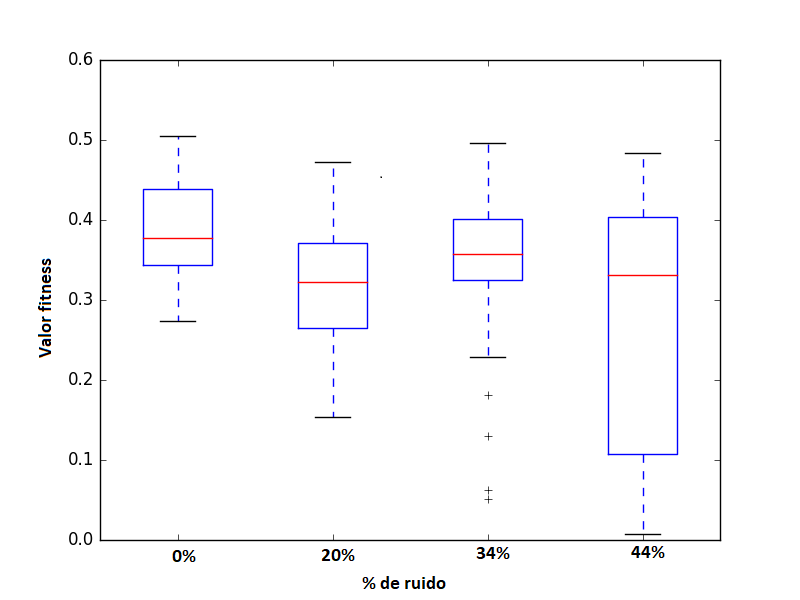
\includegraphics[width=0.8\textwidth,height=8cm]{Imagenes/BoxPlotNP2}
    \caption{Diagramas de caja para las mediciones de la fitness en presencia de ruido en los ritmos de plasticidad de los agentes de tipo 2.}
    \label{fig:boxPlotNP2}
\end{figure}

Además, para aumentar la rigurosidad, se ha efectuado un test de \textit{t de Student} para cada par de población de mediciones, con la finalidad de comprobar si las medias de las dos poblaciones de datos examinadas (de tamaño pequeño y con distribución normal) pueden considerarse iguales. Los pares de poblaciones probados han sido: sin ruido y 0.2, sin ruido y 0.34, sin ruido y 0.44. Los resultados del test pueden verse en la tabla \ref{table:tAgenteNP2}.

\begin{table}[H]
\centering
\begin{tabular}{llc}
\multicolumn{3}{c}{\textbf{Test t-Student para Agente 2}}                                                                                                    \\ \hline
\multicolumn{2}{l|}{\textbf{\begin{tabular}[c]{@{}l@{}}Población de mediciones\\ comparadas\end{tabular}}} & \multicolumn{1}{l}{\textbf{p-valor obtenido}}   \\ \hline
\multicolumn{2}{l}{Sin ruido - 0.2}                                                                        & 0.001                                            \\
\multicolumn{2}{l}{Sin ruido - 0.34}                                                                       & 0.0347                                            \\
\multicolumn{2}{l}{Sin ruido - 0.44}                                                                       & 0.00041
\end{tabular}
\caption{P-valores obtenidos de la ejecución del test \textit{t de Student} sobe los pares de poblaciones de mediciones obtenidas.}
\label{table:tAgenteNP2}
\end{table}

Al obtener, para todos los pares de poblaciones, un \textit{p-valor} menor que $0.05$ se rechaza la hipótesis de que las medias pueden considerarse iguales y por tanto, se asume que el ruido en los ritmos de plasticidad afecta negativamente a la puntuación fitness para los agentes de tipo 2.

Por último, se ha aplicado ruido a los pesos de las conexiones sinápticas de las neuronas, durante el proceso de plasticidad, guardando los valores fitness resultantes de ejecutar el experimento con presencia de dicho ruido. Los niveles de ruido probados,
de nuevo, han sido de 0, 0.2, 0.34 y 0.44. Para cada nivel de ruido se han medido 30 puntuaciones fitness. Estas mediciones se han representado en forma de diagramas de caja para visualizar su distribución (figura \ref{fig:boxPlotNW2}).

\begin{figure}[H]
    \centering
    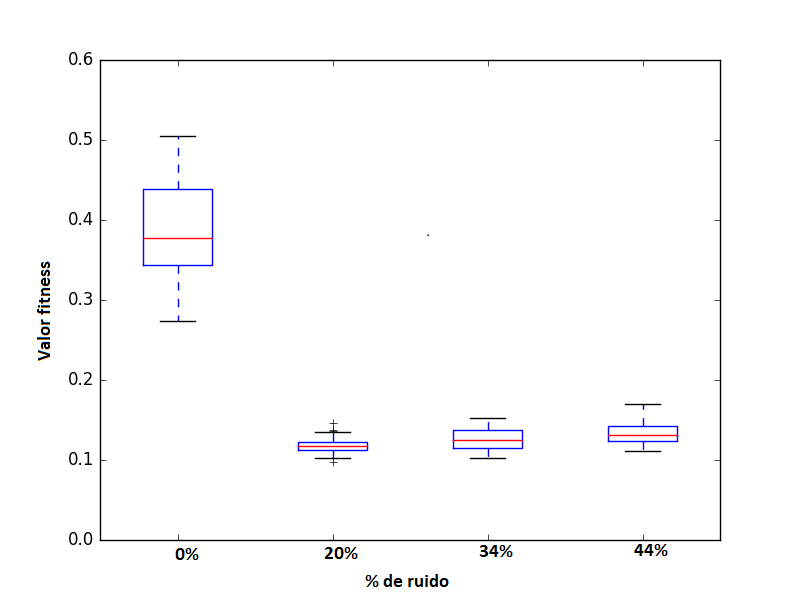
\includegraphics[width=0.8\textwidth,height=8cm]{Imagenes/BoxPlotNW2}
    \caption{Diagramas de caja para las mediciones de la fitness en presencia de ruido en los pesos sinápticos de los agentes de tipo 2.}
    \label{fig:boxPlotNW2}
\end{figure}

De nuevo, para aumentar la rigurosidad, se ha efectuado un test de \textit{t de Student} para cada par de población de mediciones, para comprobar si las medias de las dos poblaciones de datos examinadas (de tamaño pequeño y con distribución normal) pueden considerarse iguales.
Los pares de poblaciones probados han sido: sin ruido y 0.2, sin ruido y 0.34, sin ruido y 0.44. Los resultados del test pueden verse en la tabla \ref{table:tAgenteNW2}.

\begin{table}[H]
\centering
\begin{tabular}{llc}
\multicolumn{3}{c}{\textbf{Test t-Student para Agente 2}}                                                                                                    \\ \hline
\multicolumn{2}{l|}{\textbf{\begin{tabular}[c]{@{}l@{}}Población de mediciones\\ comparadas\end{tabular}}} & \multicolumn{1}{l}{\textbf{p-valor obtenido}}   \\ \hline
\multicolumn{2}{l}{Sin ruido - 0.2}                                                                        & $\sim$ 0.0                                          \\
\multicolumn{2}{l}{Sin ruido - 0.34}                                                                       & $\sim$ 0.0                                           \\
\multicolumn{2}{l}{Sin ruido - 0.44}                                                                       & $\sim$ 0.0
\end{tabular}
\caption{P-valores obtenidos de la ejecución del test \textit{t de Student} sobe los pares de poblaciones de mediciones obtenidas.}
\label{table:tAgenteNW2}
\end{table}

Al obtener, para todos los pares de poblaciones, un \textit{p-valor} menor que $0.05$ se rechaza la hipótesis de que las medias pueden considerarse iguales y por tanto, se asume que el ruido en los pesos sinápticos afecta de manera significativa a la puntuación
de los agentes de tipo 2.
